\documentclass[12pt]{article}
\usepackage{amsmath, amssymb, amsthm}
\usepackage{mathtools}
\usepackage{graphicx}
\usepackage{float}
\usepackage{hyperref}
\usepackage{xcolor}
\usepackage{listings}
\usepackage{geometry}
\usepackage{algorithm}
\usepackage{algpseudocode}
\usepackage{tikz}
\usepackage{longtable}
\usepackage{circuitikz}
\usepackage{comment}
\usepackage{MnSymbol}
\usepackage{physics}
\usepackage{booktabs}
\usepackage[section]{placeins}


\title{Design and Implementation of a Mod-7 Asynchronous Counter using T Flip-Flops}
\author{EE24BTECH11024 Abhimanyu Koushik Garimella\\EE24BTECH11002 Agamjot Singh\\IIT Hyderabad}
\date{\today}

\begin{document}

\maketitle

\section{Aim}
To design and implement a Mod-7 Asynchronous Counter using T Flip-Flops (constructed from JK Flip-Flops) and to demonstrate its performance using a Cathode Ray Oscilloscope (CRO) with a clock signal generated from an Arduino, while also visualizing the counter states using LEDs.

\section{Equipment Required}
\begin{itemize}
    \item JK Flip-Flops (IC 7476) - 3 units
    \item 3-input NAND Gate (IC 7410) - 1 unit
    \item Arduino board (for clock generation and power)
    \item Cathode Ray Oscilloscope (CRO)
    \item LED - 3 units (for visual representation of counter states)
    \item Resistors (560$\Omega$) - 3 units (for LED current limiting)
    \item Breadboard and connecting wires
\end{itemize}

\section{Theory}

\subsection{T Flip-Flop}
A T (Toggle) Flip-Flop is a digital circuit that changes its output state (toggles) when triggered by a clock pulse if its T input is set to 1. If T=0, the flip-flop maintains its previous state. The characteristic equation of a T flip-flop is:
\begin{equation}
Q_{next} = Q \oplus T
\end{equation}

\begin{align*}
\begin{array}{|c|c|c|}
\hline
T & Q_n & Q_{n+1} \\
\hline
0 & 0 & 0 \\
\hline
0 & 1 & 1 \\
\hline
1 & 0 & 1 \\
\hline
1 & 1 & 0 \\
\hline
\end{array}
\end{align*}

\subsection{JK Flip-Flop as T Flip-Flop}
A JK Flip-Flop can be configured as a T Flip-Flop by connecting both J and K inputs to the same signal (T). When J=K=1, the flip-flop toggles with each clock pulse, which is the behavior of a T flip-flop with T=1.

\begin{figure}[!ht]
\centering
\resizebox{0.6\textwidth}{!}{%
\begin{circuitikz}
\tikzstyle{every node}=[font=\LARGE]

\draw  (4.25,12.5) rectangle (8.75,7.75);
\draw (4.25,11.5) to[short] (2.75,11.5);
\node at (4.25,11.5) [circ] {};
\node at (4.25,8.75) [circ] {};
\node at (8.75,11.5) [circ] {};
\node at (8.75,8.75) [circ] {};
\node [font=\LARGE] at (4.75,11.5) {J};
\node [font=\LARGE] at (4.75,10.25) {K};
\draw (4.25,10.25) to[short] (2.75,10.25);
\node at (4.25,10.25) [circ] {};
\draw (4.25,9.25) to[short] (4.75,8.75);
\draw (4.75,8.75) to[short] (4.25,8.25);
\node [font=\LARGE] at (5.5,8.75) {CLK};
\node [font=\LARGE] at (8.25,11.5) {Q};
\node [font=\LARGE] at (8.25,8.75) {Q'};
\draw (2.75,11.5) to[short] (2.75,10.25);
\draw (2.75,11) to[short] (1.25,11);
\node [font=\LARGE] at (0.75,11) {T};
\draw (4.25,8.75) to[short] (1.25,8.75);
\draw [ dashed] (2,13.25) rectangle  (10.75,7.25);
\draw (8.75,11.5) to[short] (12,11.5);
\draw (8.75,8.75) to[short] (12,8.75);
\end{circuitikz}
}%
\caption{Constructing T Flipflop using JK Flipflop}
\end{figure}
\FloatBarrier

\subsection{Asynchronous Counter}
In an asynchronous counter, the flip-flops do not change states simultaneously. The output of one flip-flop serves as the clock input for the next flip-flop. This creates a ripple effect where the clock propagates through the counter, hence the name "ripple counter."

\subsection{Mod-7 Counter}
A Mod-7 counter cycles through 7 states (from 0 to 6) before resetting. For a binary counter, we need 3 flip-flops to represent states 0 to 6 (000 to 110 in binary). To ensure the counter resets after state 6 (110) and skips state 7 (111), we implement a reset mechanism using a NAND gate.\newline 
All the outputs ($Q_1$, $Q_2$, $Q_3$) are connected to a 3-input NAND gate and the output of the NAND gate is connected to the clear pin of the flipflop. When state 7 (111) is attained, the ouput of the NAND gate is 0 and state is switched to 0 (000) instead of 7 immediately.

\section{Circuit and Timing Diagram}

\begin{figure}[!ht]
\centering
\resizebox{1\textwidth}{!}{%
\begin{circuitikz}
\tikzstyle{every node}=[font=\large]
\draw  (6,15.75) rectangle (9.25,11);
\draw  (12.25,15.75) rectangle (15.5,11);
\draw  (18.75,15.75) rectangle (22,11);
\draw (6,15) to[short] (5,15);
\draw (5,15) to[short] (5,16.75);
\draw (12.25,15) to[short] (11,15);
\draw (11,15) to[short] (11,16.75);
\draw (18.75,15) to[short] (17.5,15);
\draw (17.5,15) to[short] (17.5,16.75);
\draw (9.25,13.5) to[short] (10.75,13.5);
\draw (10.75,13.5) to[short] (10.75,12.5);
\draw (10.75,12.5) to[short] (12.25,12.5);
\draw (15.5,13.75) to[short] (17,13.75);
\draw (17,13.75) to[short] (17,12.5);
\draw (17,12.5) to[short] (18.75,12.5);
\draw (3.75,12.5) to[short] (6,12.5);
\draw (22,12.5) to[short] (23.25,12.5);
\draw (23.75,12.5) to[short] (23.75,10);
\draw (23.75,10) to[short] (22.25,10);
\draw (17.25,10.75) to[short] (22.75,10.75);
\draw (23.25,10.75) to[short] (23.25,10.25);
\draw (23.25,10.25) to[short] (22.25,10.25);
\draw (17,12.5) to[short] (17,10.75);
\draw (17,10.75) to[short] (18.25,10.75);
\draw (10.75,12.5) to[short] (10.75,9.25);
\draw (10.75,9.25) to[short] (23.25,9.25);
\draw (23.75,9.25) to[short] (23.75,9.75);
\draw (23.75,9.75) to[short] (22.25,9.75);
\draw (22.5,10.25) to[short] (22.5,10.25);
\draw (22.5,9.75) to[short] (22.5,9.75);
\draw (22.5,10.25) node[ieeestd nand port, anchor=in 2, scale=0.89, rotate=180](port){} (port.out) to[short] (20.5,10);
\draw (port.left) to[short] (22.5,10);
\draw (22.5,10.75) to[short] (23.25,10.75);
\draw (23,12.5) to[short] (23.75,12.5);
\draw (23.25,9.25) to[short] (23.75,9.25);
\draw (20.5,11) to[short] (20.5,10);
\draw (14.25,11) to[short] (14.25,10);
\draw (14.25,10) to[short] (20.5,10);
\draw (8,11) to[short] (8,10);
\draw (8,10) to[short] (14.5,10);
\draw (6.75,11) to[short] (6.75,8.5);
\draw (13.25,11) to[short] (13.25,8.5);
\draw (19.5,11) to[short] (19.5,8.5);
\draw (6.75,8.5) to[short] (20.25,8.5);
%\draw (20.25,8.5) to (20.25,8.25) node[ground]{};
\draw (20.25,8.5) to[battery2] (20.25,7.5);
\draw (20.25,7) to (20.25,7.5) node[ground]{};
\draw (5,16.75) to[short] (19.5,16.75);
\draw (19.5,16.75) to[battery2] (21.5,16.75);
\draw (21.25,16.75) to (22.25,16.75) node[ground]{};
\node [font=\Large] at (7.5,13.75) {T Flipflop};
\node [font=\Large] at (14,13.75) {T Flipflop};
\node [font=\Large] at (20.5,13.75) {T Flipflop};
\node [font=\large] at (3.25,12.5) {Clk};
\node [font=\large] at (9.75,13) {$Q_1$};
\node [font=\large] at (16,13.25) {$Q_2$};
\node [font=\large] at (22.25,12.75) {$Q3$};
\node [font=\large] at (10.5,17.25) {$T = 1$};
\node [font=\large] at (6.75,11.25) {Preset};
\draw [short] (6.25,11.5) -- (7.25,11.5);
\node [font=\large] at (8,11.25) {Clear};
\node [font=\Large] at (5.5,14.5) {T};
\node [font=\Large] at (18,14.5) {T};
\node [font=\Large] at (11.75,14.5) {T};
\draw [short] (7.5,11.5) -- (8.5,11.5);
\node [font=\large] at (13,11.25) {Preset};
\draw [short] (12.5,11.5) -- (13.5,11.5);
\node [font=\large] at (14.25,11.25) {Clear};
\draw [short] (13.75,11.5) -- (14.75,11.5);
\node [font=\large] at (19.5,11.25) {Preset};
\draw [short] (19,11.5) -- (20,11.5);
\node [font=\large] at (20.75,11.25) {Clear};
\draw [short] (20.25,11.5) -- (21.25,11.5);
\node [font=\large] at (11.75,12) {Clk};
\node [font=\large] at (18.25,13) {Clk};
\end{circuitikz}
}%

\label{counter}
\caption{Implementation of a Mod-7 Asynchronous Ripple Counter}
\end{figure}
\FloatBarrier

\begin{figure}
    \centering
    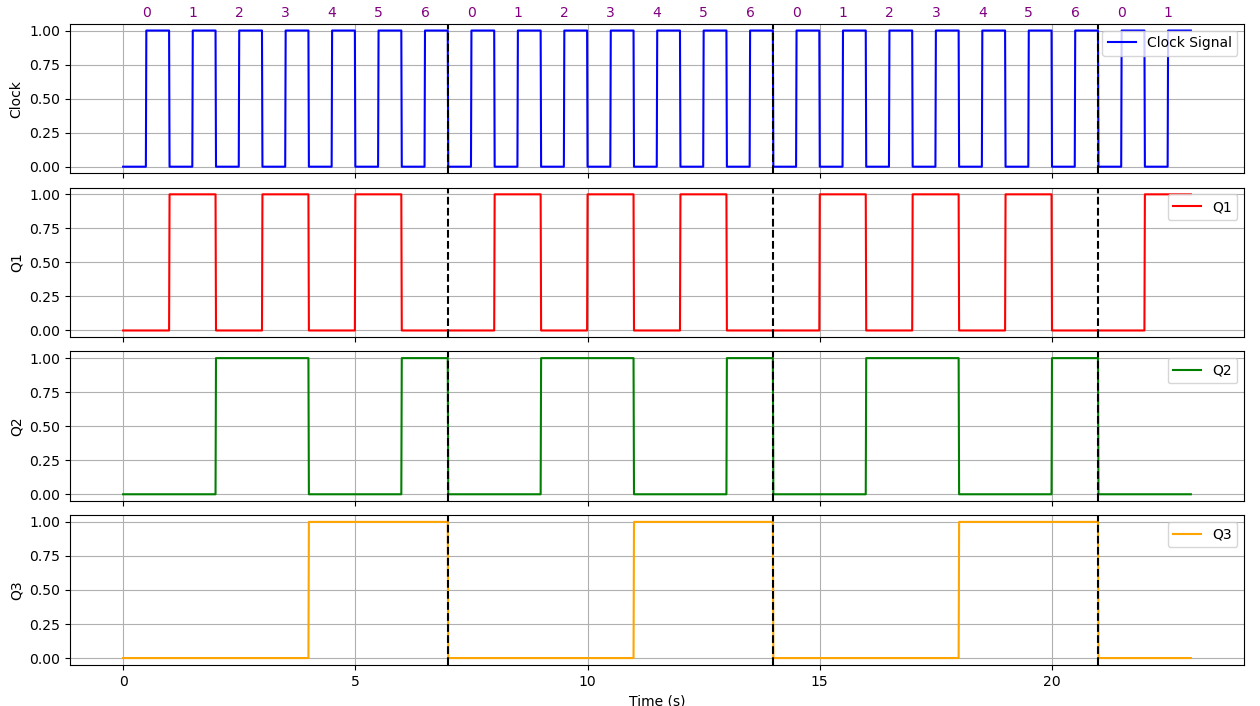
\includegraphics[width=1\linewidth]{./figs/Tcounter.png}
    \caption{Timing Diagrams of Clock and all three outputs ($Q_1$, $Q_2$, $Q_3$)}
    \label{fig:enter-label}
\end{figure}
\FloatBarrier

\section{Procedure}

\begin{enumerate}
    \item Configure the JK flip-flops as T flip-flops by connecting both J and K inputs to logic 1 (+5V).
    \item Connect the flip-flops in cascade, with the Q output of each flip-flop connected to the clock input of the next flip-flop.
    \item Connect the Arduino's pin 13 to the clock input of the first flip-flop (FF0).
    \item Connect the Q outputs of all three flip-flops (Q0, Q1, Q2) to the inputs of the 3-input NAND gate (7410).
    \item Connect the output of the NAND gate to the $\overline{\text{CLEAR}}$ pins of all flip-flops.
    \item Connect the $\overline{\text{PRESET}}$ pins of all flip-flops to power (+5V).
    \item Connect LEDs with current-limiting resistors to the Q outputs of each flip-flop for visual state representation.
    \item Connect the Q outputs of all flip-flops to the CRO channels for visualization.
    \item Program the Arduino to generate a square wave clock signal (code provided below).
    \item Power up the circuit and observe the LED states and waveforms on the CRO.
    \item Verify that the counter cycles through states 0 to 6 and then resets to 0.
\end{enumerate}

\subsection{Arduino Code for Clock Generation}
\begin{verbatim}
void setup() {
  pinMode(13, OUTPUT);  // Set pin 13 as output
}

void loop() {
  digitalWrite(13, LOW);  // Set pin 13 LOW
  delay(500);             // Wait for 500 milliseconds
  digitalWrite(13, HIGH); // Set pin 13 HIGH
  delay(500);             // Wait for 500 milliseconds
}
\end{verbatim}
\FloatBarrier

This generates a clock signal with time period $= 1$s.

\section{Results}
\subsection{LED States}
\begin{figure*}[!htb]
    {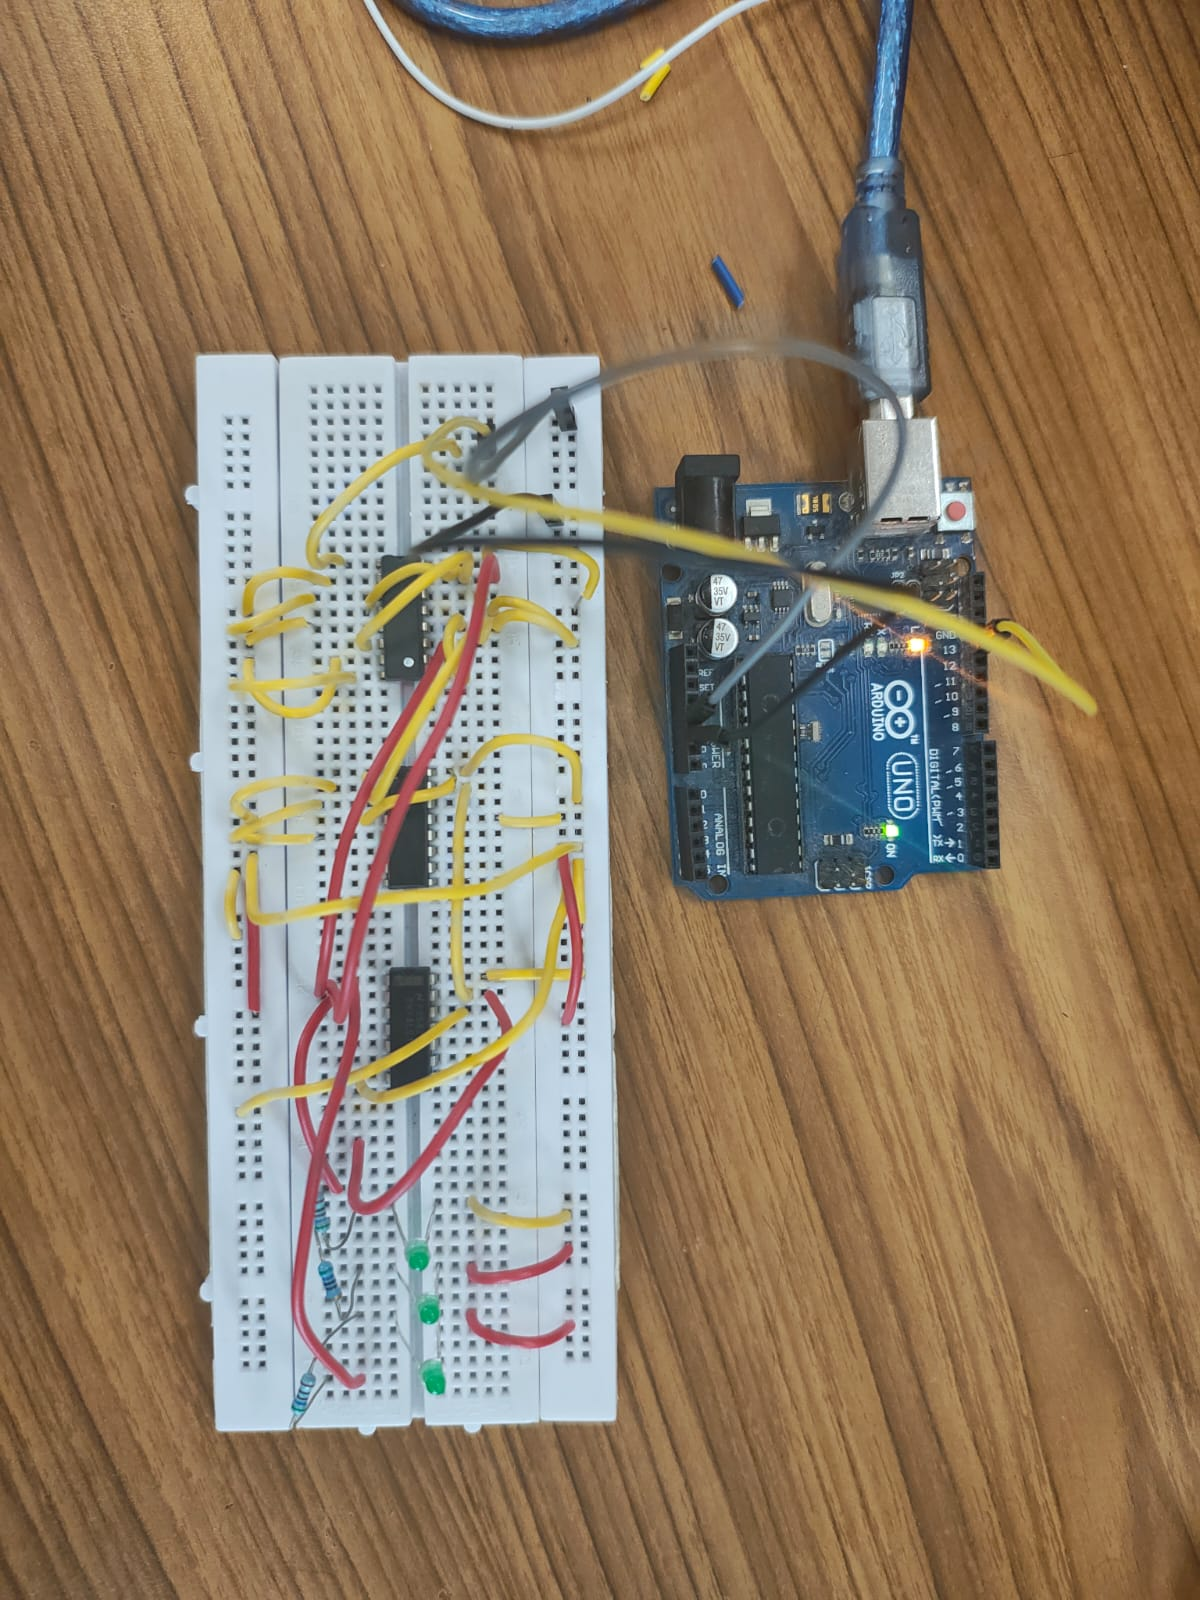
\includegraphics[ width=0.4\textwidth,angle=90]{./figs/counter_0.jpeg}}
    \hspace{\fill}
    {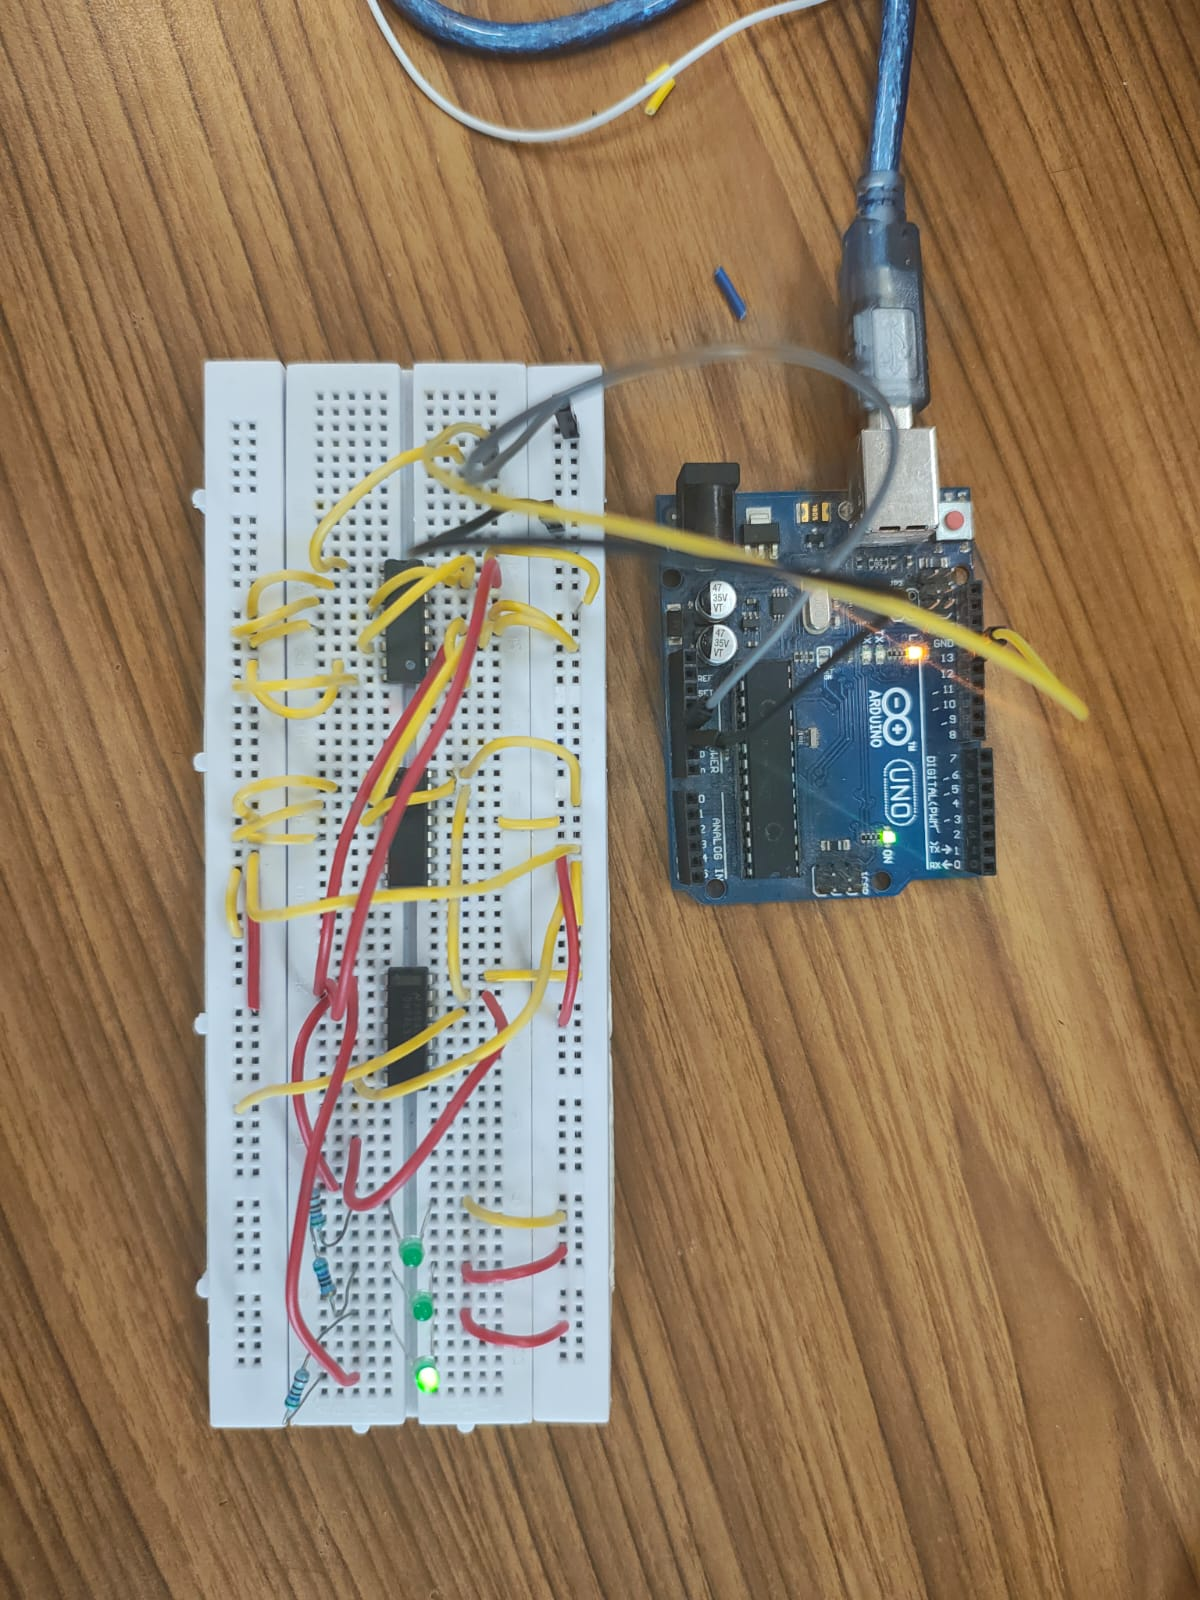
\includegraphics[ width=0.4\textwidth,angle=90]{./figs/counter_1.jpeg}}
    \caption{State 0 and 1}
\end{figure*}
\FloatBarrier

\begin{figure*}[!htb]
    {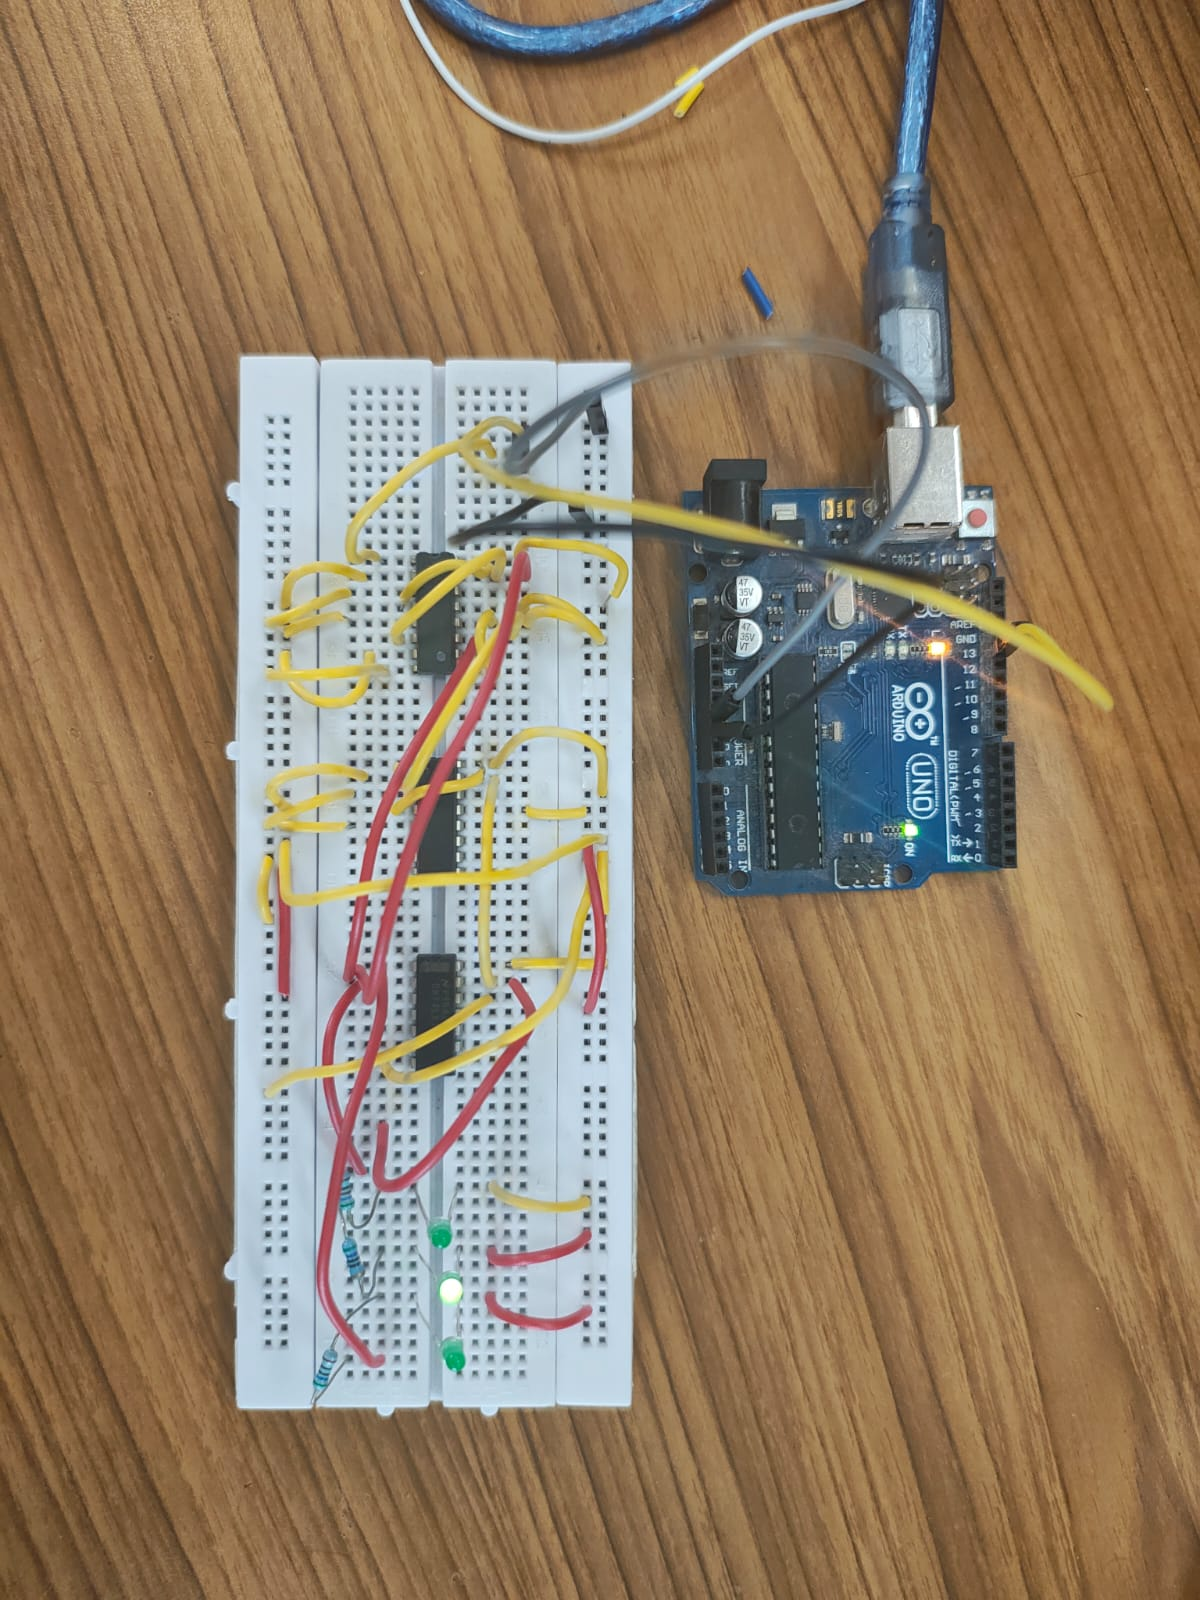
\includegraphics[ width=0.4\textwidth,angle=90]{./figs/counter_2.jpeg}}
    \hspace{\fill}
    {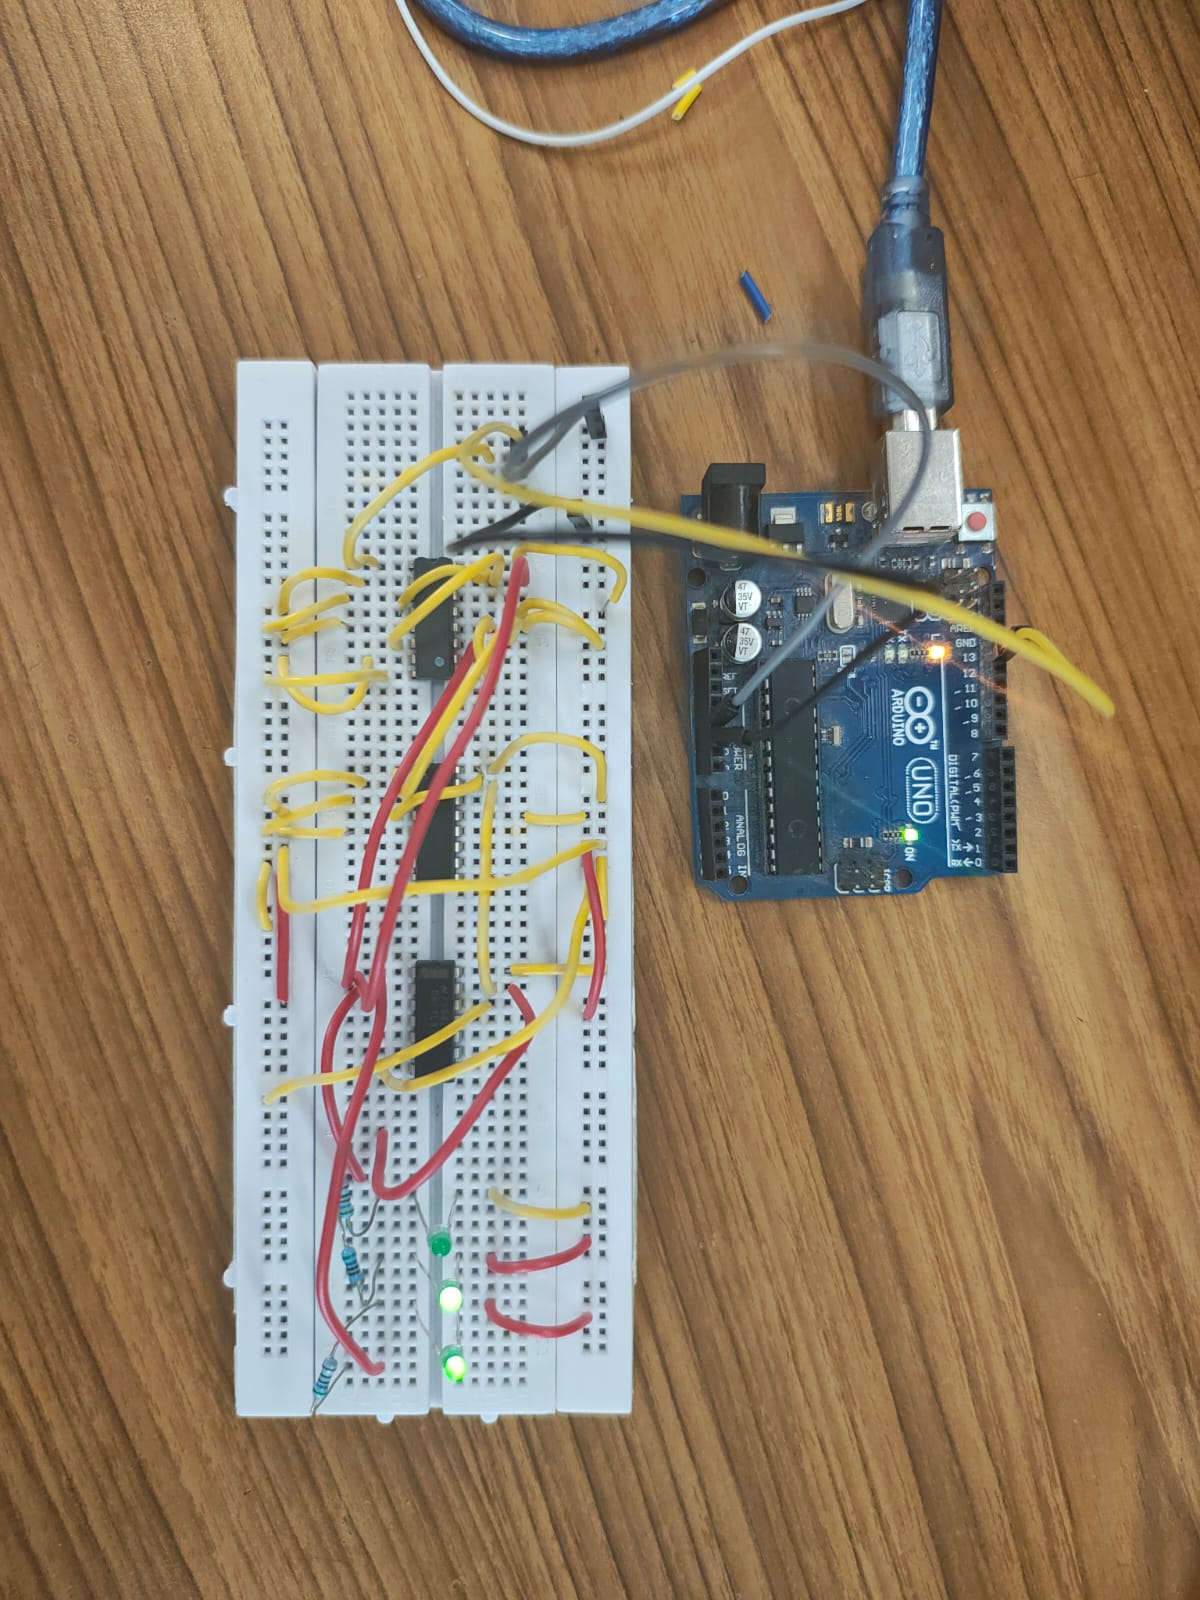
\includegraphics[ width=0.4\textwidth,angle=90]{./figs/counter_3.jpeg}}
    \caption{State 2 and 3}
\end{figure*}
\FloatBarrier

\begin{figure*}[!htb]
    {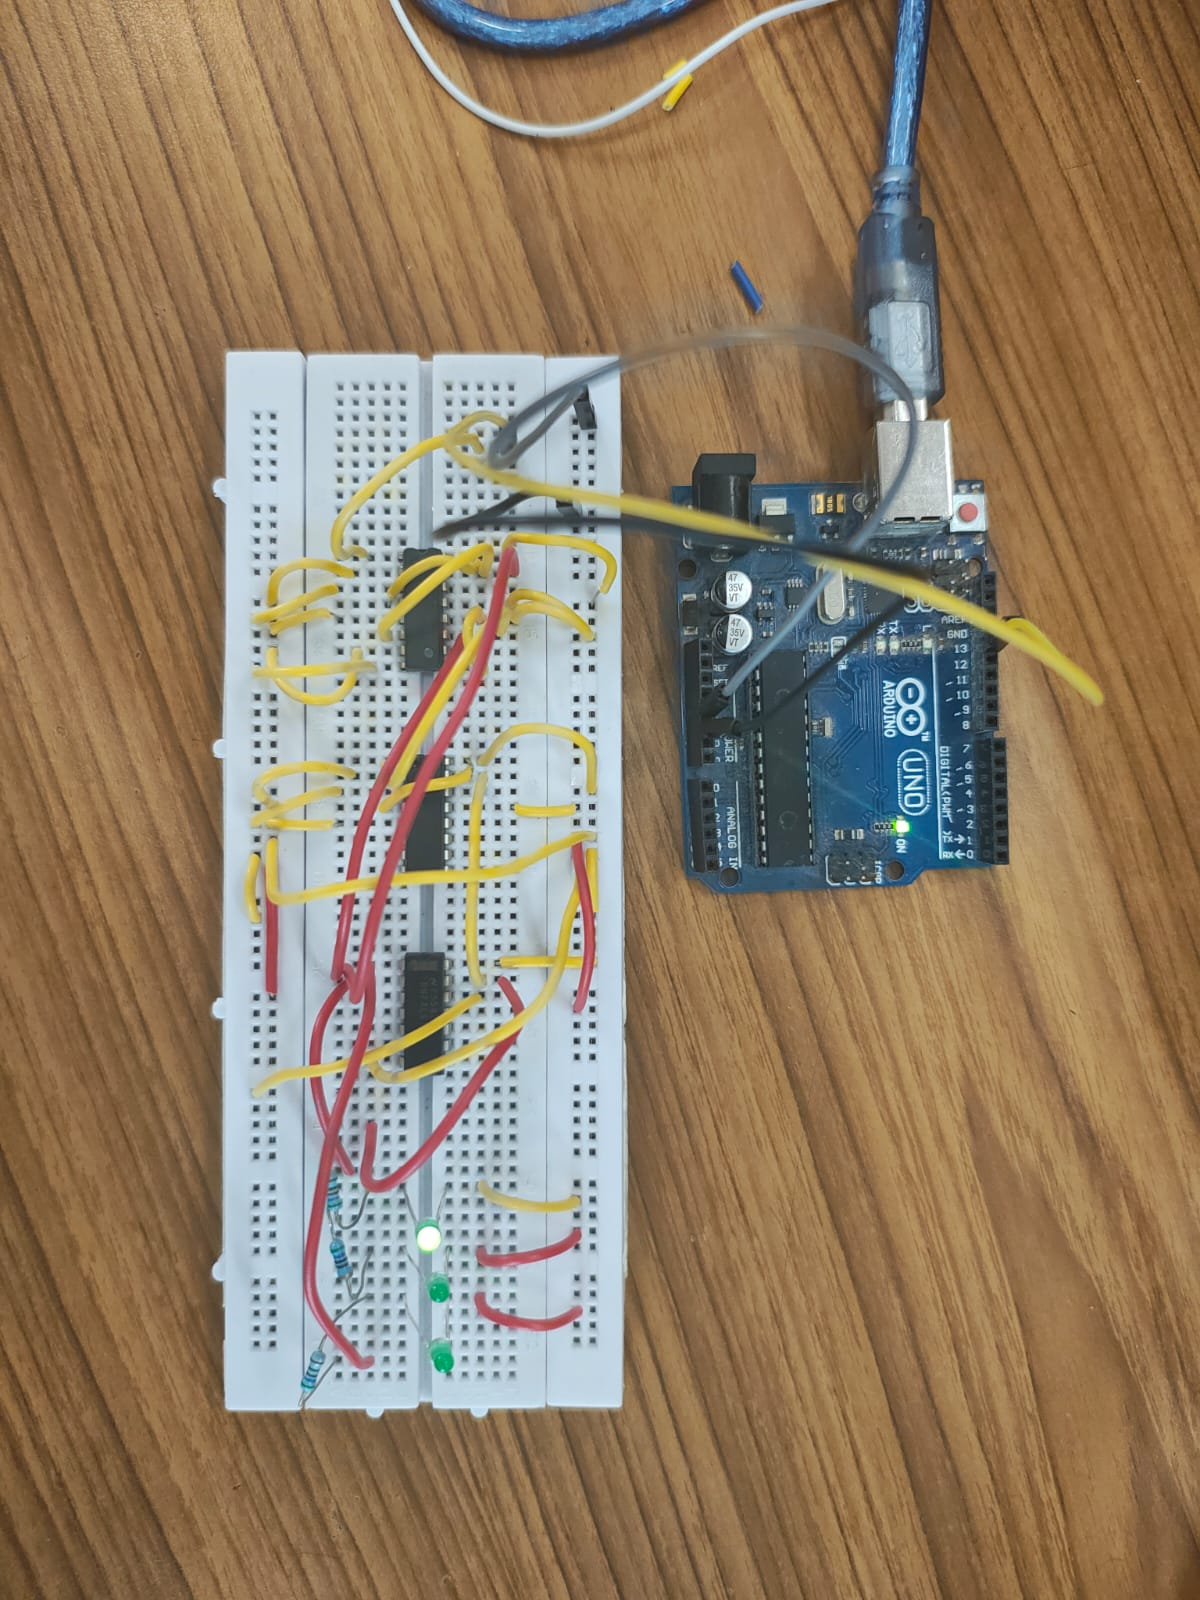
\includegraphics[ width=0.4\textwidth,angle=90]{./figs/counter_4.jpeg}}
    \hspace{\fill}
    {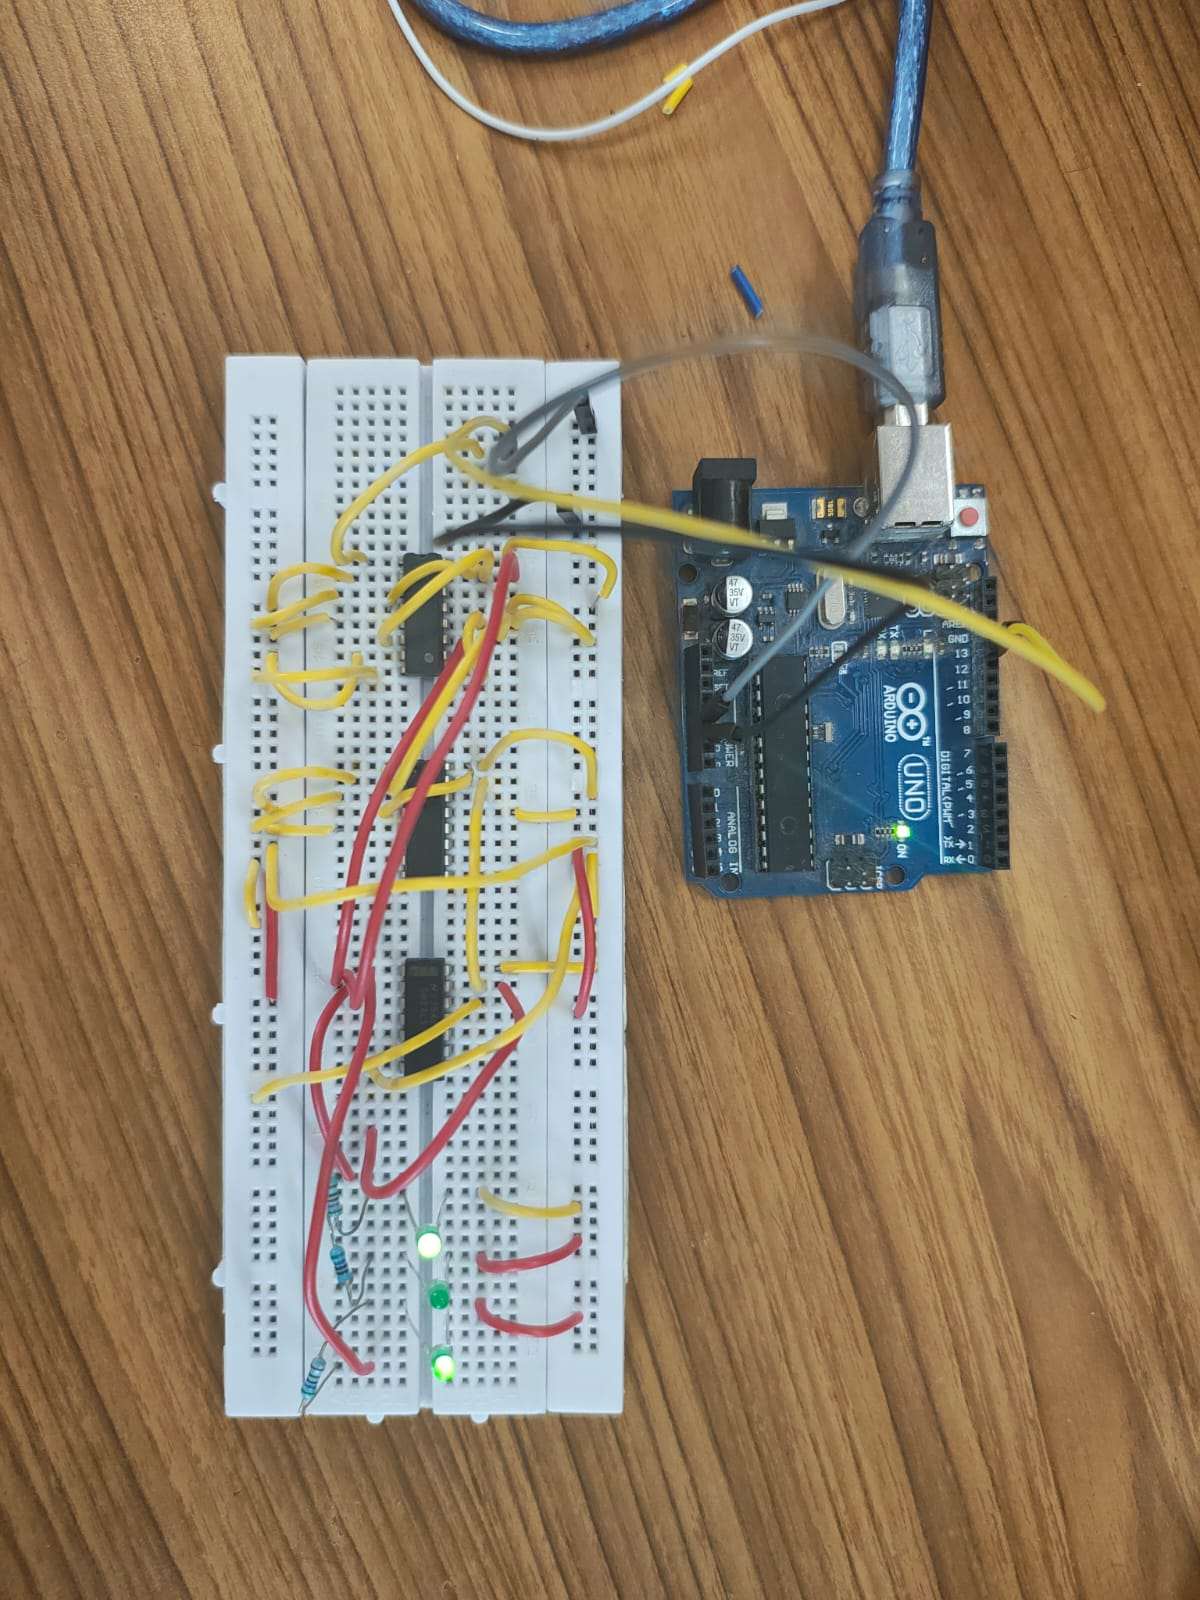
\includegraphics[ width=0.4\textwidth,angle=90]{./figs/counter_5.jpeg}}
    \caption{State 4 and 5}
\end{figure*}
\FloatBarrier

\begin{figure*}[!htb]
    {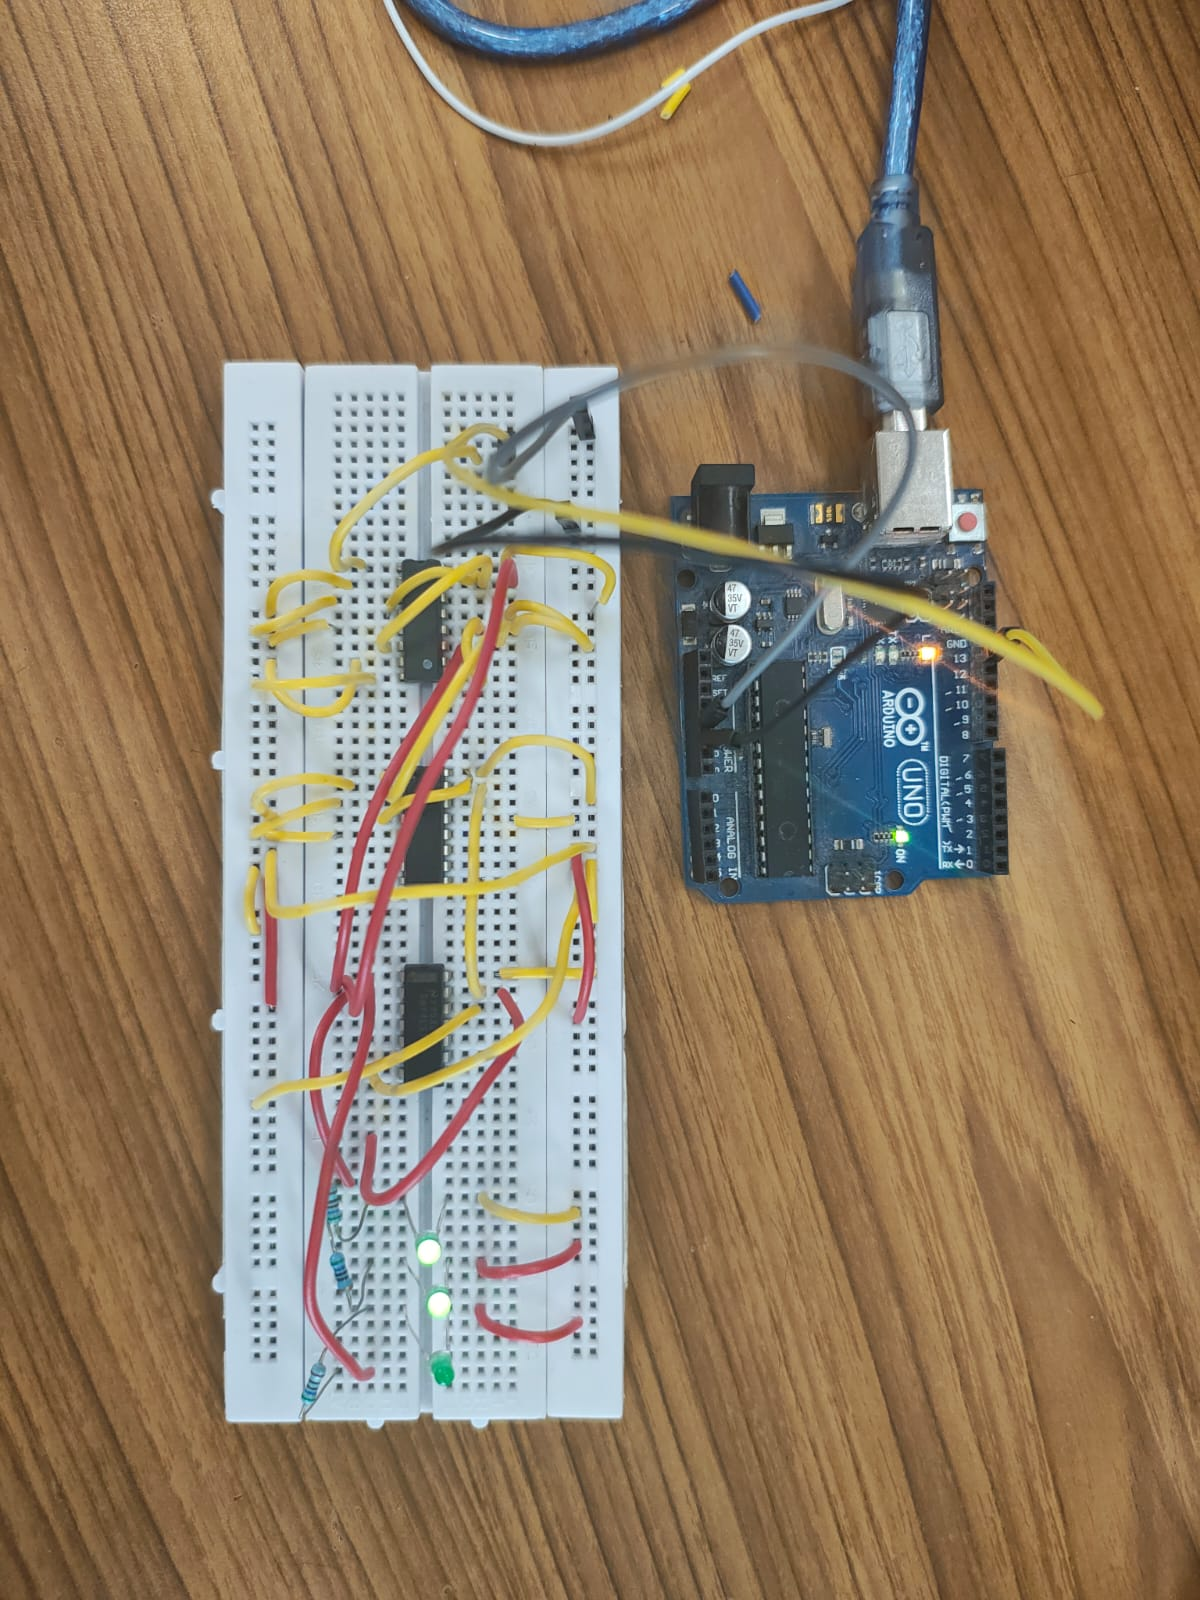
\includegraphics[ width=0.4\textwidth,angle=90]{./figs/counter_6.jpeg}}
    \hspace{\fill}
    {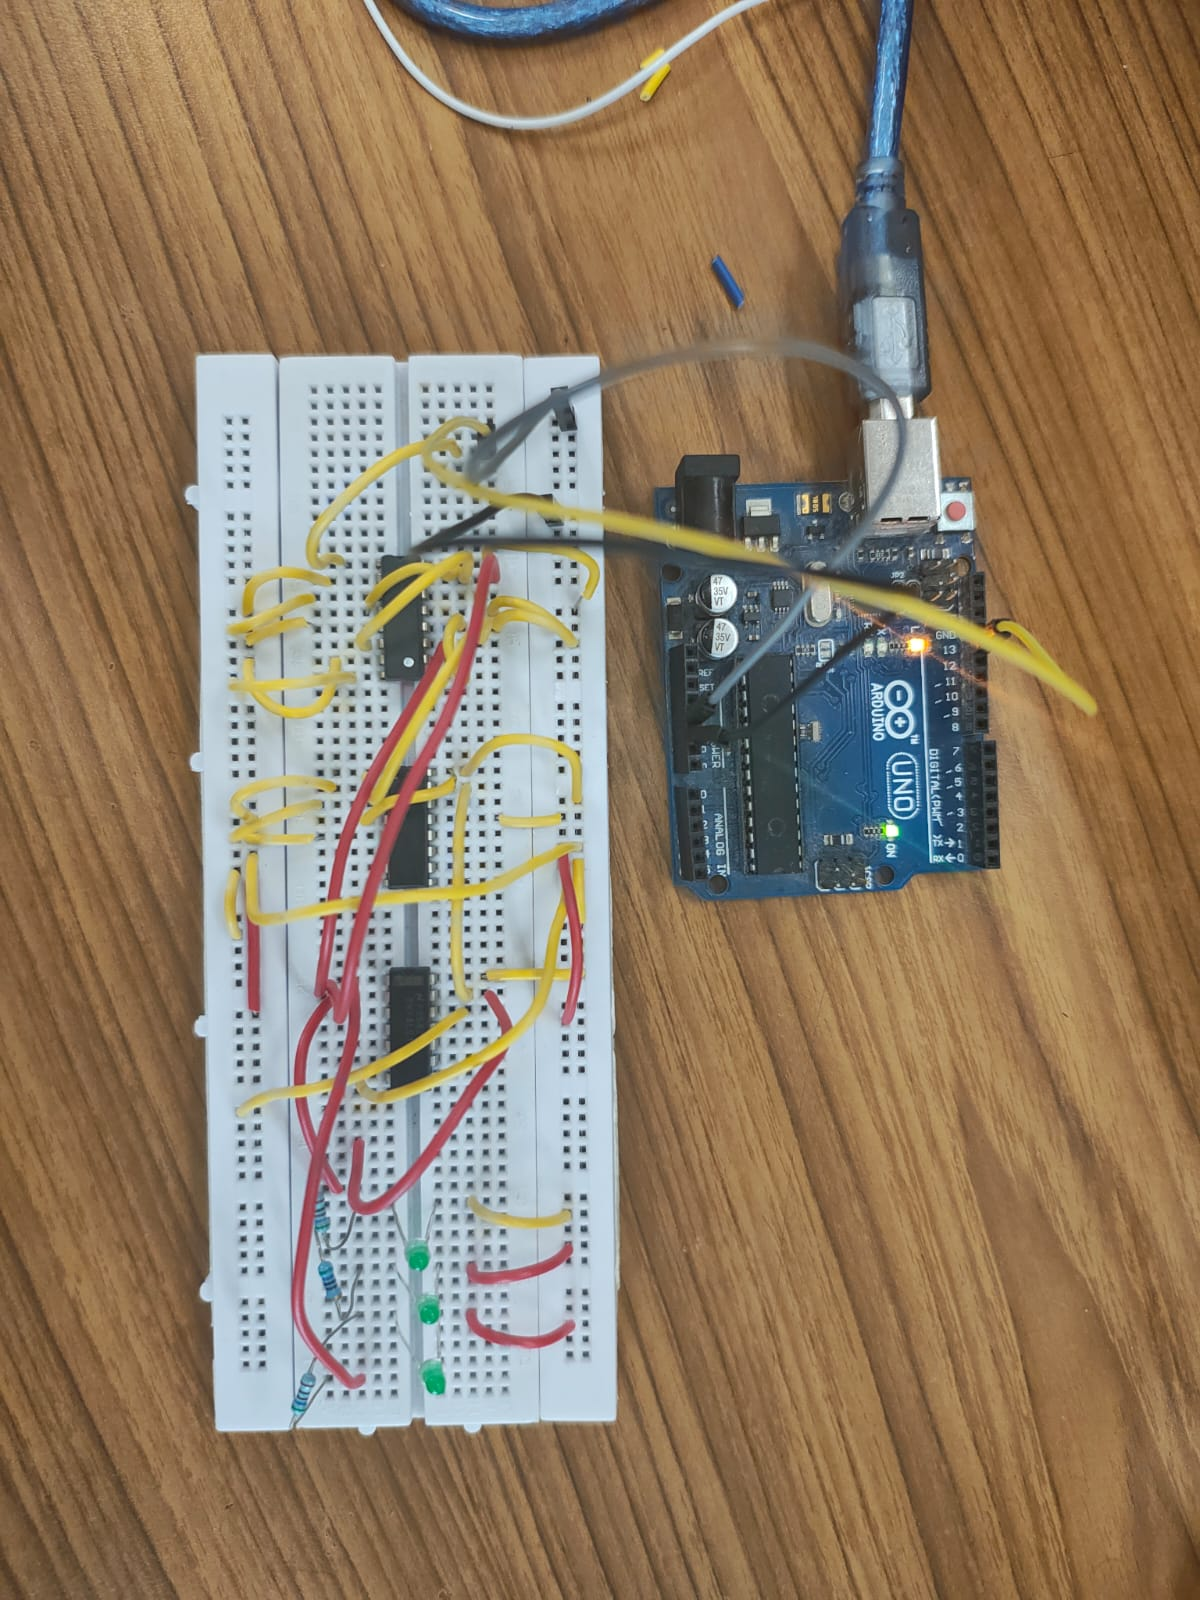
\includegraphics[ width=0.4\textwidth,angle=90]{./figs/counter_0.jpeg}}
    \caption{State 6 and back to 0}
\end{figure*}
\FloatBarrier

\subsection{Oscilloscope Readings}
\begin{figure*}[!htb]
    \centering
    {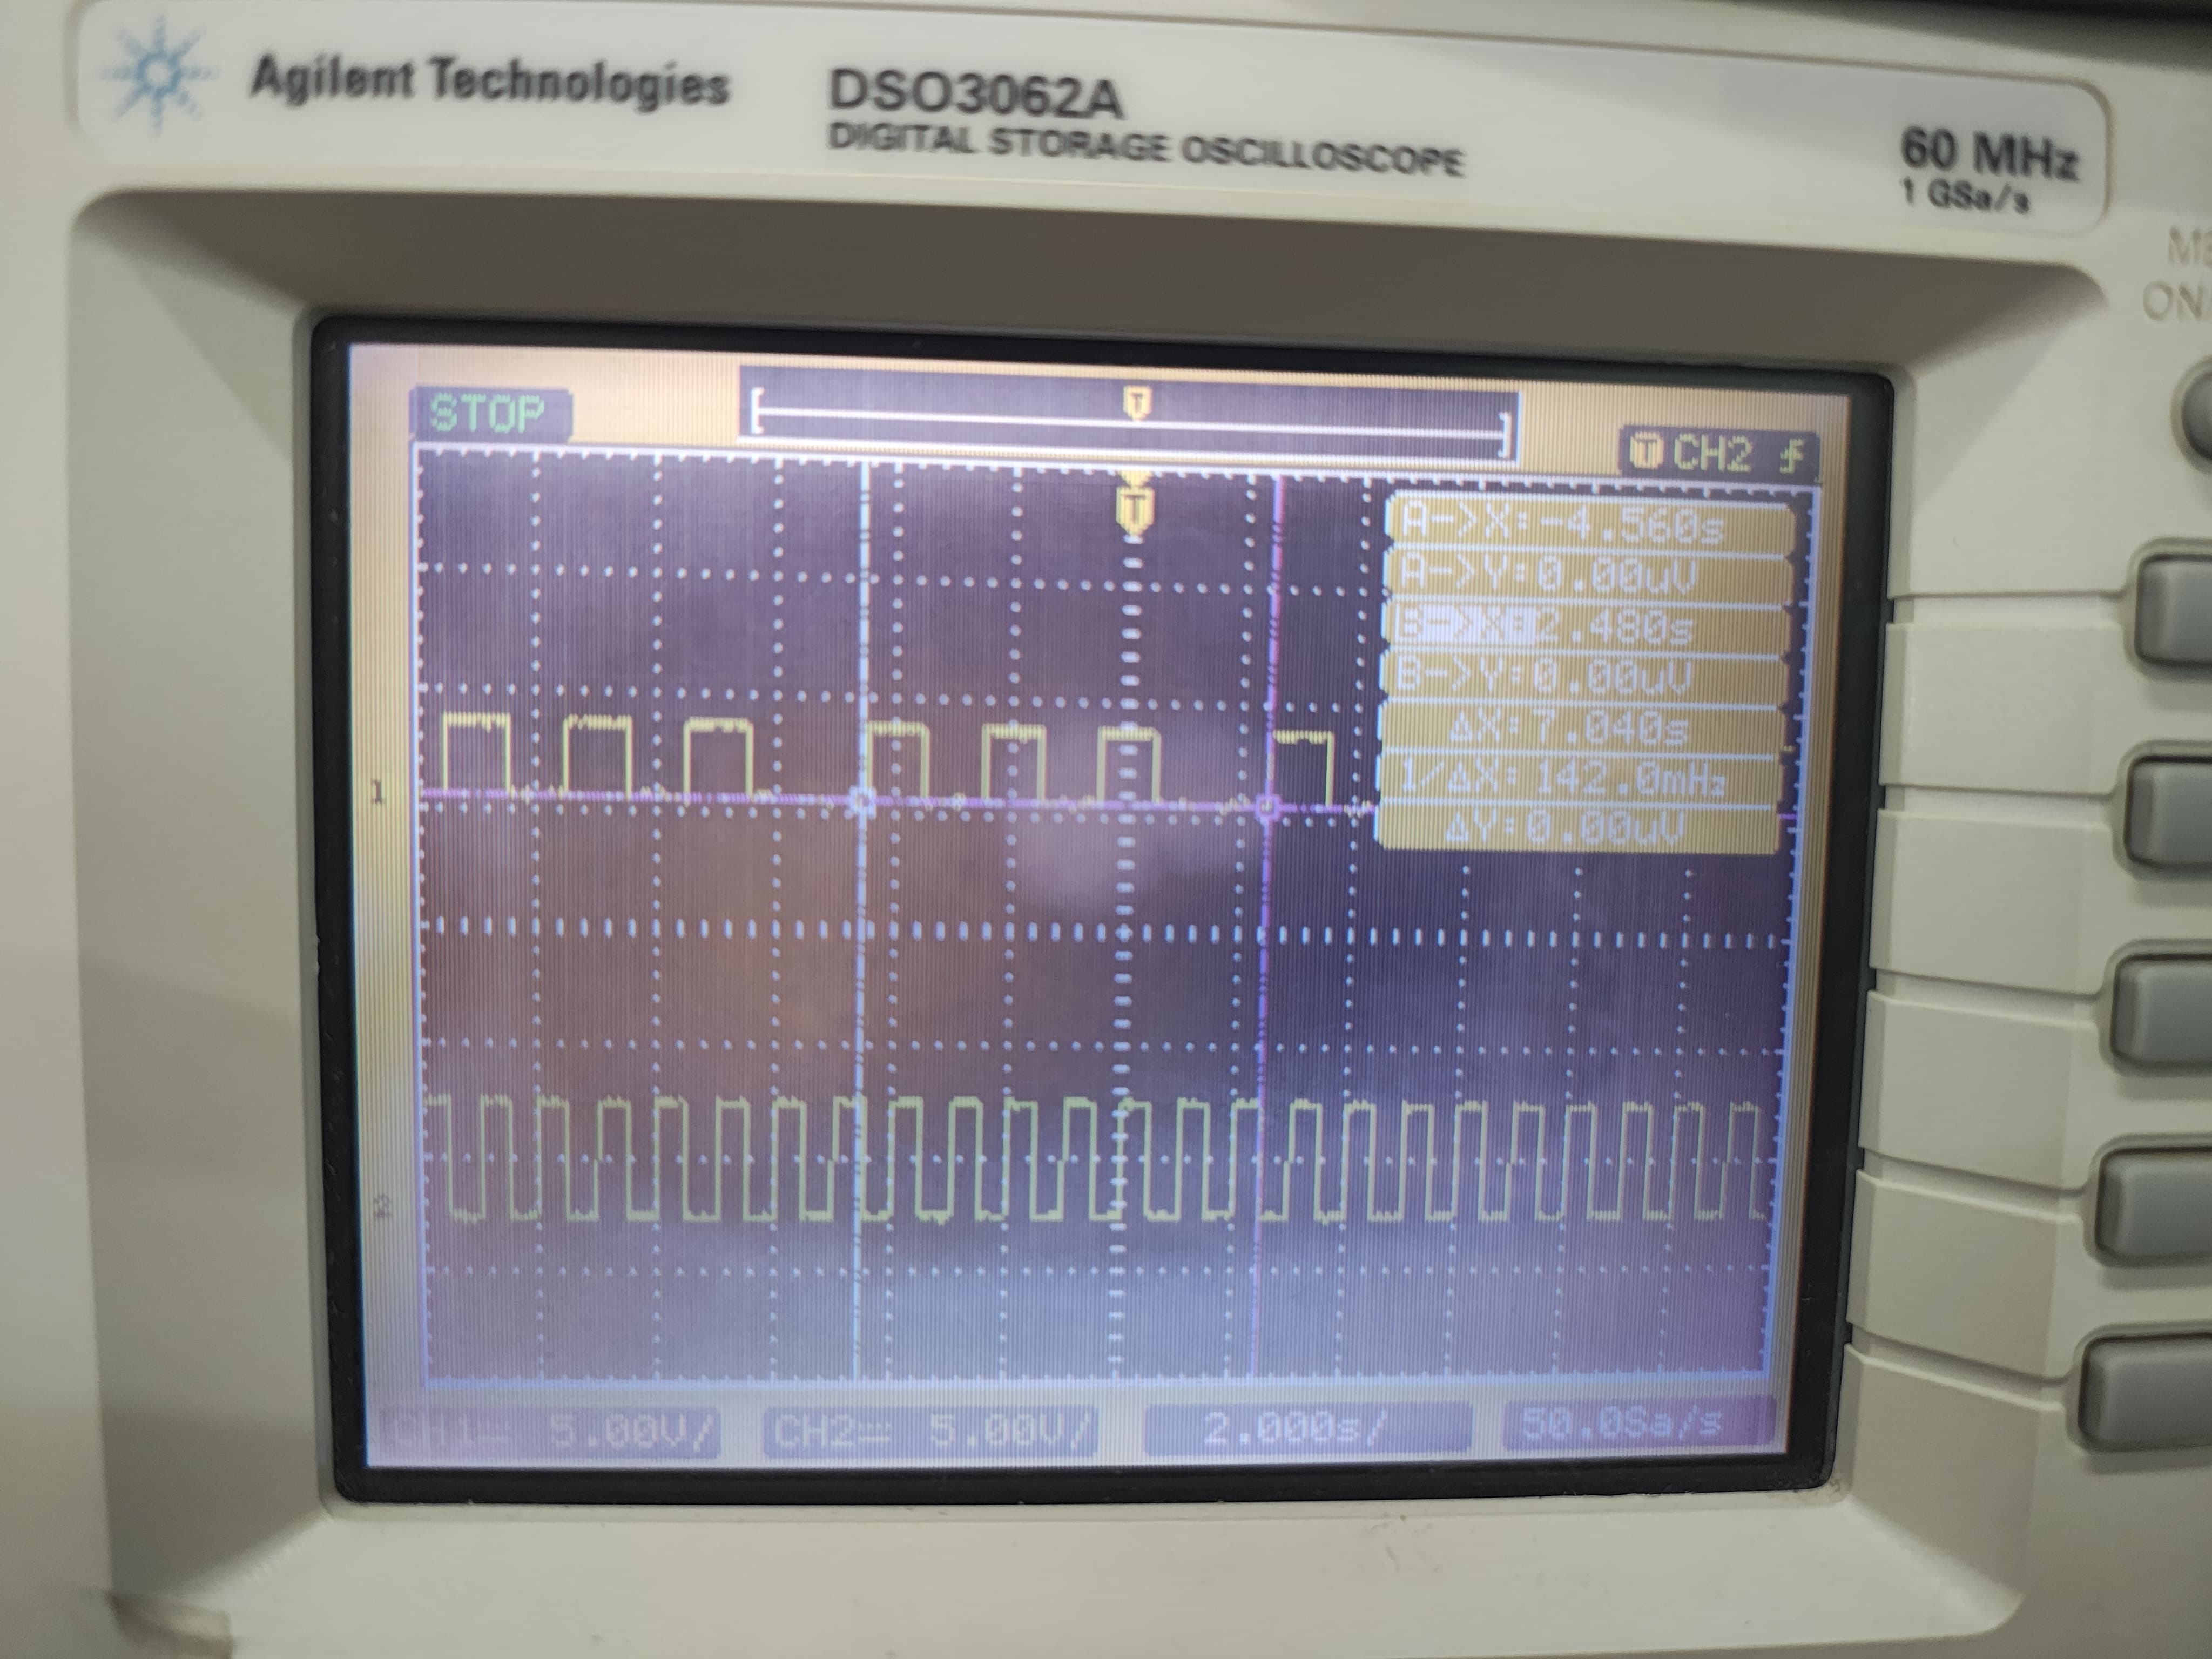
\includegraphics[ width=0.7\textwidth]{./figs/cro_1.jpeg}}
    \caption{Reading of $Q_1$ vs Clock}
\end{figure*}

\begin{figure*}[!htb]
    \centering
    {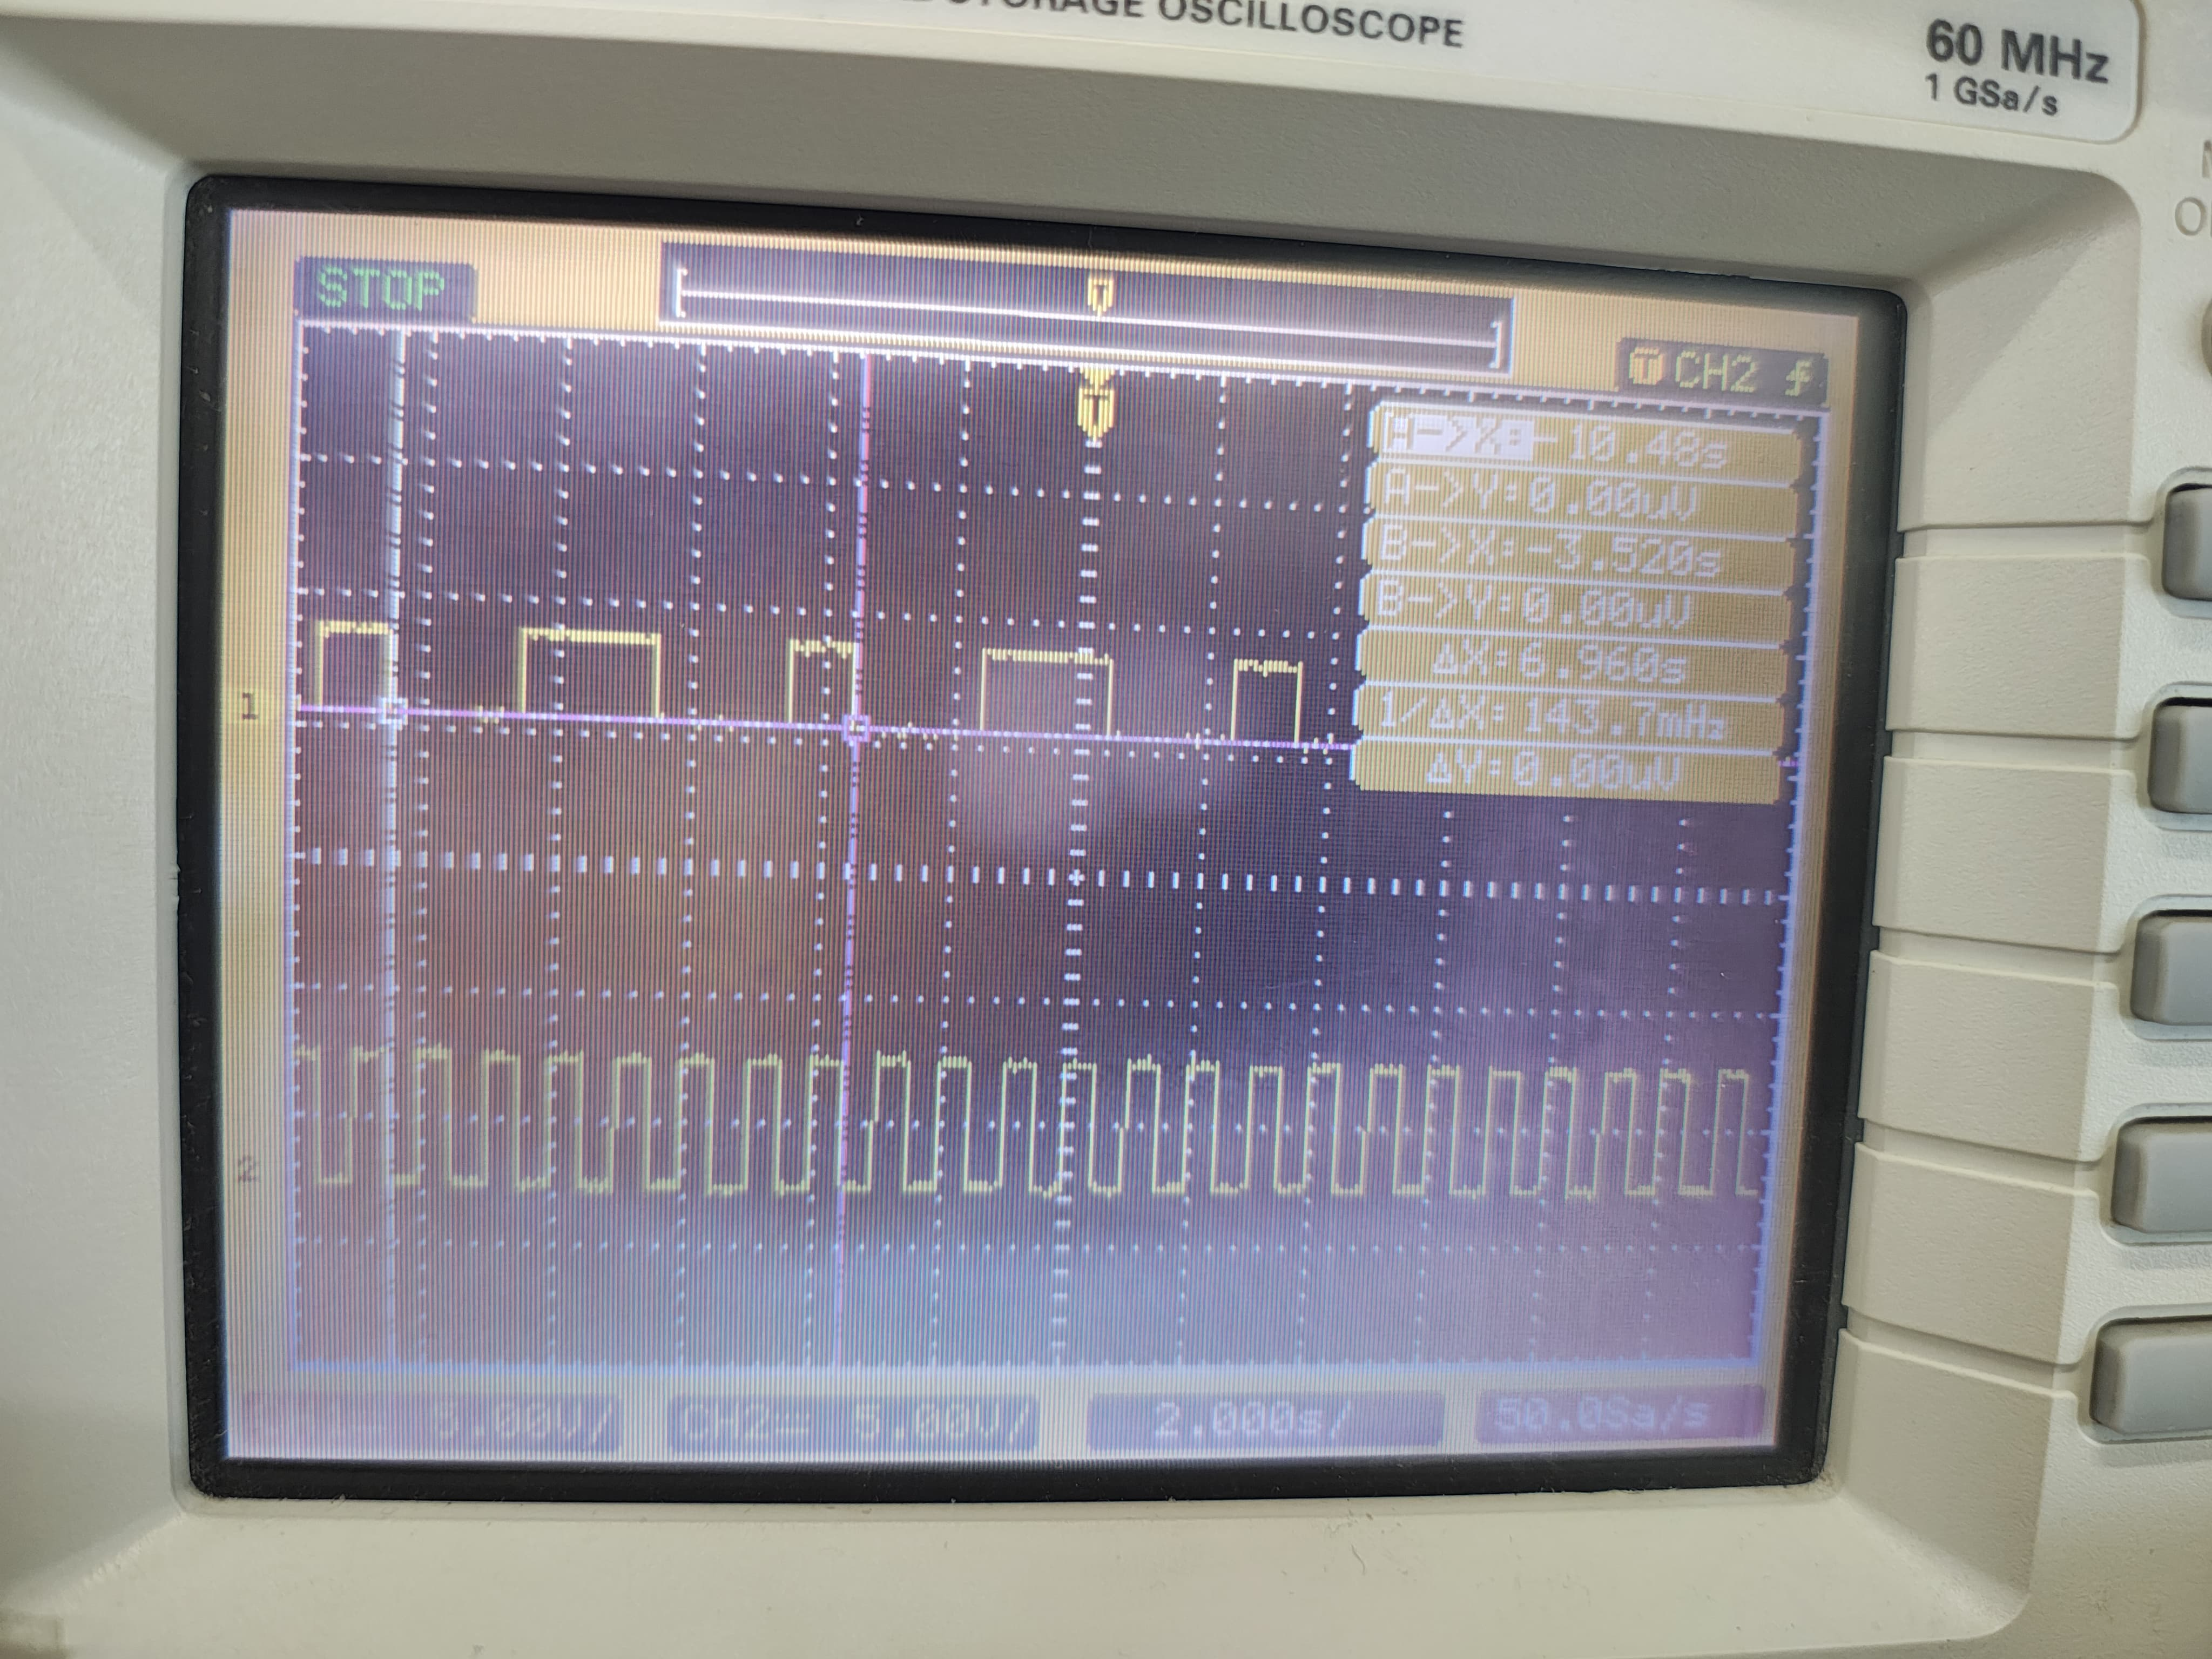
\includegraphics[ width=0.7\textwidth]{./figs/cro_2.jpeg}}
    \caption{Reading of $Q_2$ vs Clock}
\end{figure*}

\begin{figure*}[!htb]
    \centering
    {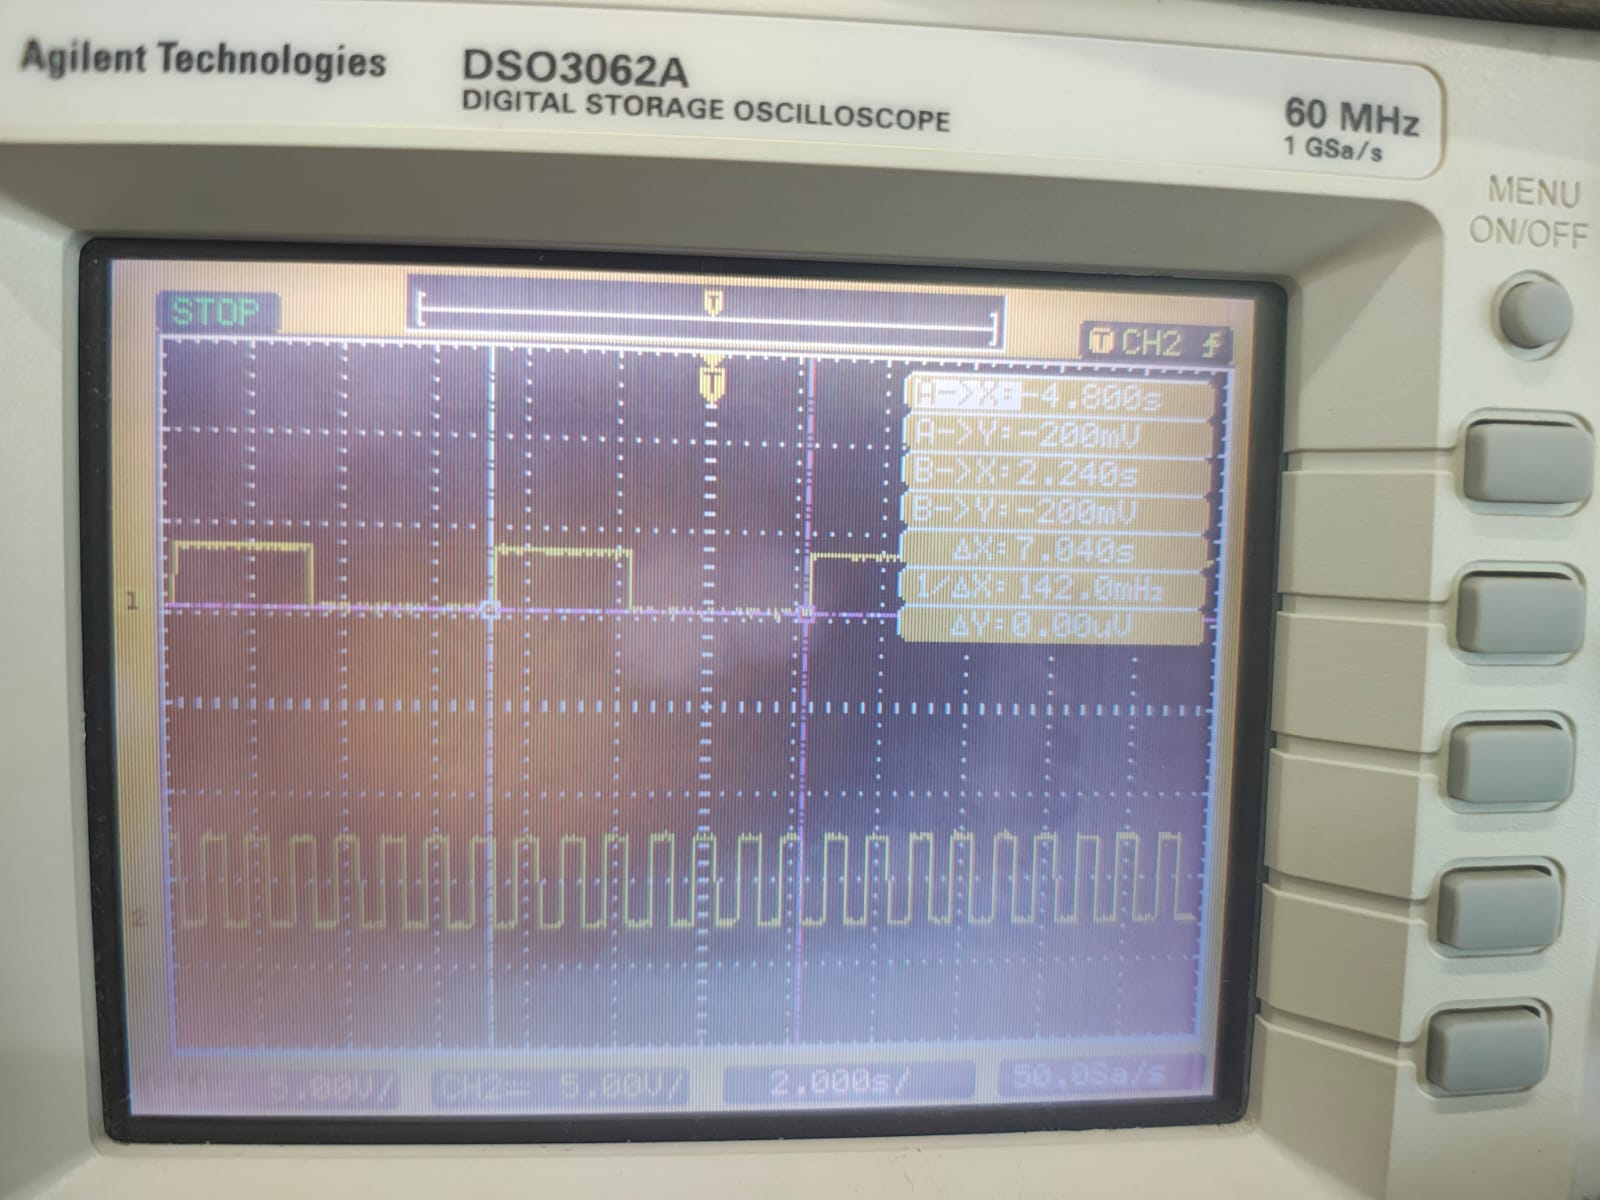
\includegraphics[ width=0.7\textwidth]{./figs/cro_3.jpeg}}
    \caption{Reading of $Q_3$ vs Clock}
\end{figure*}

\section{Observation}

The counter was observed to cycle through the following states:

\begin{table}[H]
\centering
\begin{tabular}{cccccc}
\toprule
\textbf{Count} & \textbf{Q2} & \textbf{Q1} & \textbf{Q0} & \textbf{Decimal Equivalent} & \textbf{LED State} \\
\midrule
0 & 0 & 0 & 0 & 0 & Off-Off-Off \\
1 & 0 & 0 & 1 & 1 & Off-Off-On \\
2 & 0 & 1 & 0 & 2 & Off-On-Off \\
3 & 0 & 1 & 1 & 3 & Off-On-On \\
4 & 1 & 0 & 0 & 4 & On-Off-Off \\
5 & 1 & 0 & 1 & 5 & On-Off-On \\
6 & 1 & 1 & 0 & 6 & On-On-Off \\
7 & 0 & 0 & 0 & 0 (Reset) & Off-Off-Off \\
\bottomrule
\end{tabular}
\caption{State Sequence of Mod-7 Counter with LED Indications}
\label{tab:states}
\end{table}

On the CRO, the following waveforms were observed:
\begin{itemize}
    \item $Q_0$: Square wave with the time period $= 7$s
    \item $Q_1$: Square wave also with the time period $= 7$s
    \item $Q_2$: Square wave also with the time period $= 7$s
\end{itemize}

The NAND gate output remained HIGH during states 0 through 6. When the counter attempted to enter state 7 (111), the NAND gate output went LOW momentarily, clearing all flip-flops and resetting the counter to state 0 (000).

The LEDs provided a visual representation of the counter states, with each LED corresponding to a bit in the counter (Q0, Q1, Q2). This allowed for easy verification of the counter's operation without the need for measurement equipment.

\section{Conclusion}

The Mod-7 asynchronous counter using T flip-flops was successfully designed and implemented. The counter correctly cycled through states 0 to 6 before resetting to state 0, skipping state 7 as intended. The timing diagram observed on the CRO matched the expected behavior, confirming the proper operation of the counter.

For applications requiring precise timing, synchronous counters would be more appropriate to eliminate the propagation delay issues inherent in asynchronous designs. However, the simplicity and ease of implementation of asynchronous counters make them suitable for many practical applications where slight timing discrepancies are acceptable.

\end{document}

